
In Geometron we view symbols as being any geometry with meaning, including physical constructions and sequences of actions.  A ``printer'' refers to any machine which prints a symbol in this generalized sense.  This means printer now refers to a huge class of machines, really any machine with automation can be thought of as a generalized printer of symbols.  When we create symbols with the Geometron language, using the Geometron Hypercube and the Geometron Virtual Machine, we are building sequences of geometric actions, which can call other actions to build up complex fractal constructions.  One of the kinds of actions we can build into this are discrete movements of machines, just as we use discrete movements of a virtual machine when the cursor moves around on the screen building two dimensional graphics in a web browser.

\begin{figure}
	\centering
	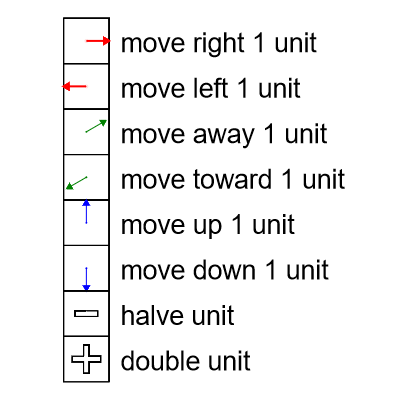
\includegraphics[width=3in]{figures/machines/basicmovements.png}
	\caption[basicmovements]
	{Basic geometric actions of machine control for an arbitrary machine that moves along three perpendicular axes.}
\end{figure}

To build up control of machines for printers, we start with the most basic discrete movements.  To begin with, we discuss the control of machines that have three axes of motion, all of which are perpendicular, along the up, down, left, right, forward, and back directions.  We start with eight basic actions: a single step in each of the six directions, doubling the step size and halving the step size.  Just these eight actions are enough to position a machine with three axis in any location in the available space.  Just as binary numbers can be used to express any decimal number, this binary approach to geometry can be used to express any geometric location.  Also note that these actions are independent of scale, and have no numerical units.  A sequence of actions is all relative to some unspecified starting unit. So a glyph created to on some agricultural tool at the 100 meter scale can print at the nanometer scale using an atomic probe of some kind with no modification to the glyph in principle.  Our language is both independent of numbers and of what machine is carrying out the actions.   

\begin{figure}
	\centering
	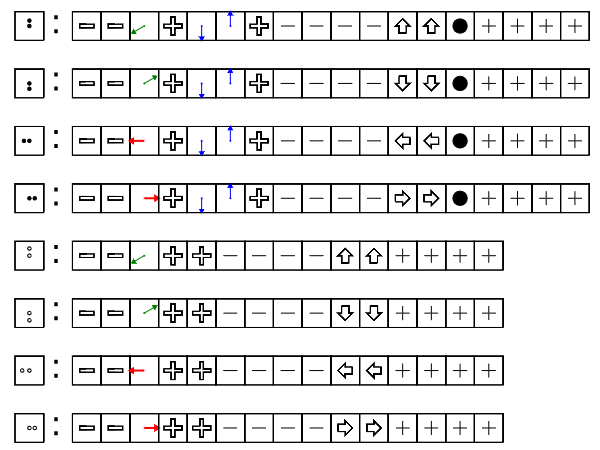
\includegraphics[width=3in]{figures/machines/actions05xx.png}
	\caption[actions05xx]
	{Dot actions from which symbols are constructed.}
\end{figure}

Recall that each action has a symbol which can be displayed in a web browser.  These symbols serve to allow us to edit glyphs which control machine action.  Glyphs like this can be used to create the shapes in the range between addresses 0500 and 0577 in the Action Cube.  These also have symbols in the Symbol Cube in addresses between 01500 and 01577.  Whole universes of complex symbols can be built in the machine action shape table. Also, the overall system can have many more types of control than documented here if there are more components with more degrees of freedom for more complex machines, again with a full 64 potential geometric actions in the other action table from address 0400 through 0477.

The main initial application of all this we will discuss here is printing out icons which are easily created and shared on the Geometron system.  This method for printing symbols in physical objects can be a powerful tool for communication with other people about any idea about which people are capable of thinking or communicating.  This printing system is based on a ``two and a half d printer'' model, in which we create three dimensional media on a two dimensional surface using a three dimensional tool to represent a two dimensional icon symbol.  We are using the word icon here in a very general sense, just as it is used on layout of software systems: it is a symbol which can be used to represent anything, much like a word.  Icons can in fact just be words, as there is a font built into the system.  We build icons on the basis of four basic actions: move up, move down, move left, move right, move up with pixel draw, down with pixel, left with pixel and right with pixel.  When a subject is chosen, we come up with a symbol for it, find that somewhere on the Web or draw it and photograph it and upload it, then align it and trace it with tools built into the Geometron system.  Icon glyphs are stored in the Icon Feed, which can be used to share text by copy and paste with anyone anywhere.  

\begin{figure}
	\centering
	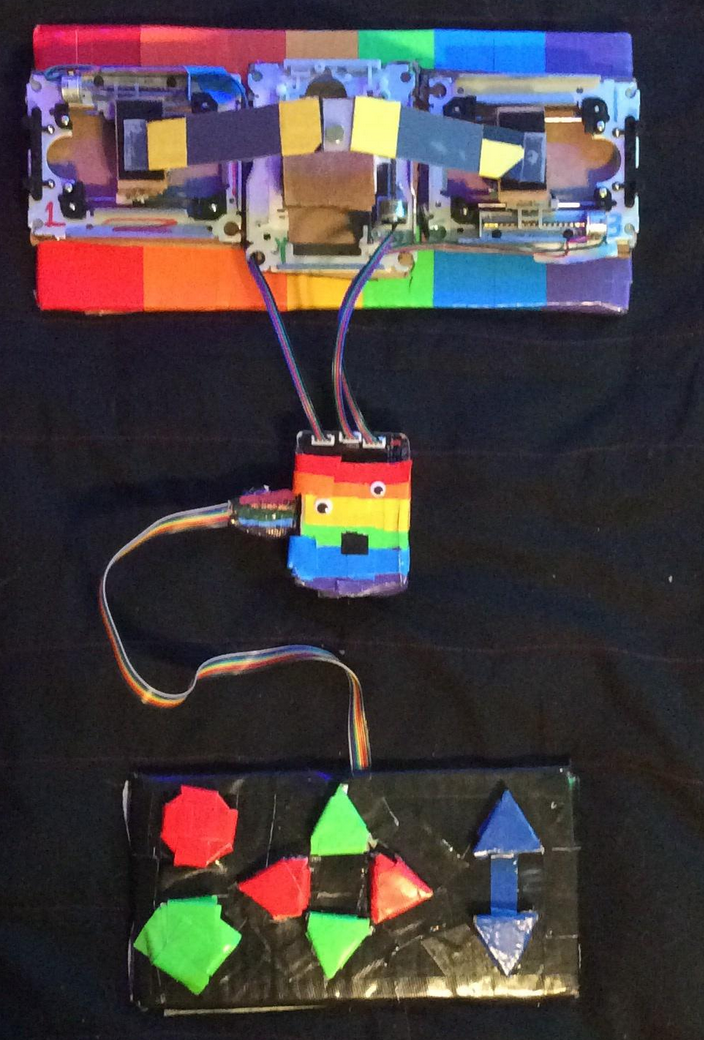
\includegraphics[width=3in]{figures/machines/printerphoto.png}
	\caption[printerphoto]
	{Clay Icon Printer.  Printer is built from 3 DVD drives, cardboard and plastic trash, duct tape, an Arduino, and some custom electronics.}
\end{figure}

\begin{figure}
	\centering
	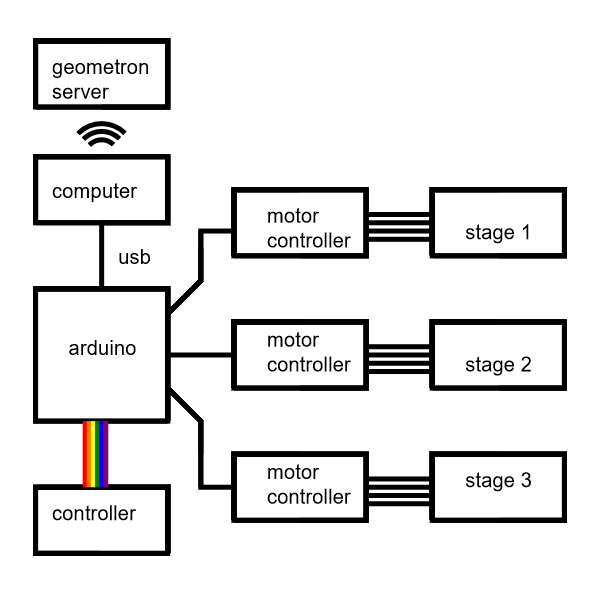
\includegraphics[width=3in]{figures/machines/printerblockdiagram.png}
	\caption[printerblockdiagram]
	{Block diagram of Trash Robot printer.  The motion stages are salvaged from DVD or CD ROM drives.  The motor drivers are off the shelf from Pololu Robotics.  The Arduino is the Arduino UNO, and the whole system including the motors gets power from the USB connected to a computer.  The computer can be used to interact with a Geoemtron server over the local network or on the global Internet to create programs which are copy/pasted into the Arduino IDE as described in the Trash Robot chapter.}
\end{figure}


We built printers from a set of 3 DVD drives, some cardboard and plastic, an Arduino and some custom electronics.  When a pixel is drawn, a tool is moved down and back up in the z direction, and if this is done with a pointy tool over clay, it can create a dimple in the surface.  The printer replicated in the Scrolls included with the system is about 14 by 5 inches, with a controller, as shown in one of the figures.  It is for printing in round bits of polymer clay between 1 and 2 inches in diameter.  Once the clay has been printed in, it can be baked in a home oven to harden it.  Because it has dimples in it for each pixel, another piece of clay molded into the original print will make a mirror copy of the icon.  When this clay is baked, it will form a stamp, which when applied to yet a third piece of clay will make a copy of the original print.  This can then be painted and sanded flat so that the pixels are now colored in.  Or it can be used to print yet another stamp.  Because an original can go to many stamps, the stamps can go to many more copies, and each copy can make many more stamps, we again have a geometric construction which can scale exponentially if there are number of people willing and able to carry out the copying action.  Icons can also be used to make .stl files to send to a 3d printer, and .svg files with smaller holes which can be sent to a laser cutter for spray paint stencils.  Since the 3d printed files also have pixels which can be pressed into an object to make molds, this is again self-replicating symbolic media.  And of course with a spray paint stencil and a can of spray paint symbol replication can be extremely rapid.  


\begin{figure}
	\centering
	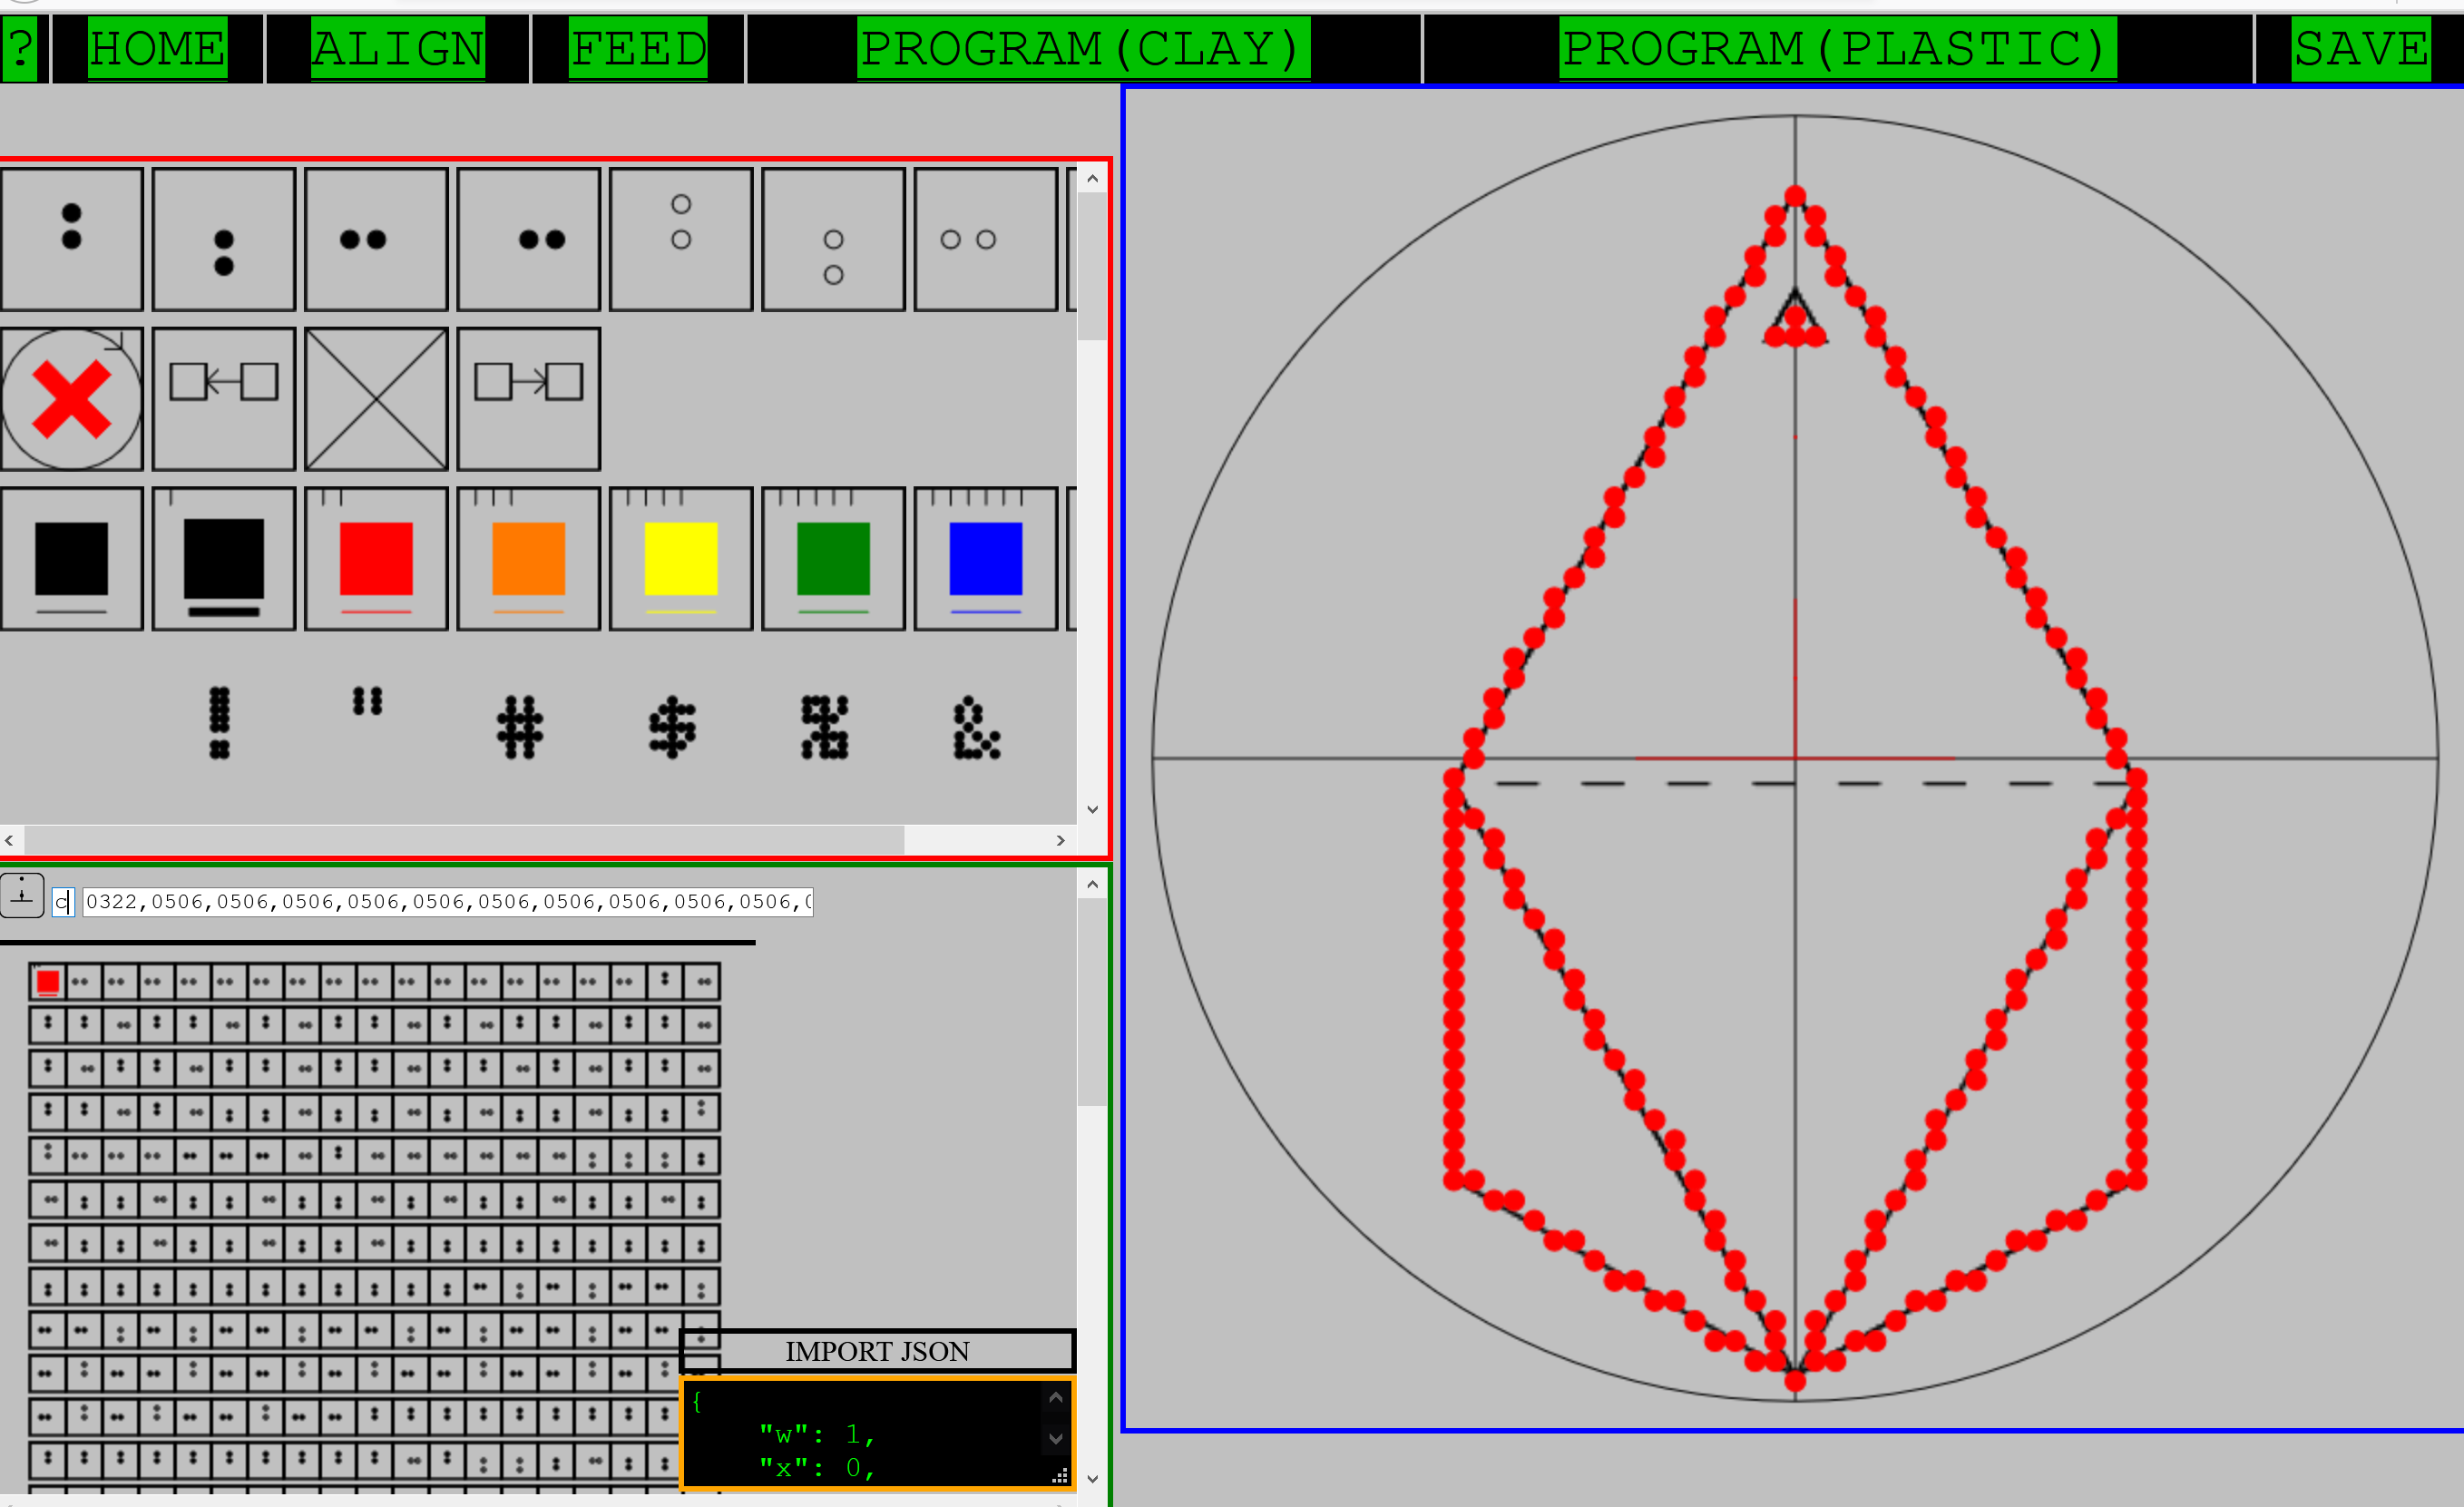
\includegraphics[width=3in]{figures/machines/trace.png}
	\caption[trace]
	{The icon tracer.  Images are put in the Image Feeds as used in the rest of the system, then aligned in the icon aligner, and traced.  When it is saved it goes into the Icon Feed for sharing with the world.}
\end{figure}

\begin{figure}
	\centering
	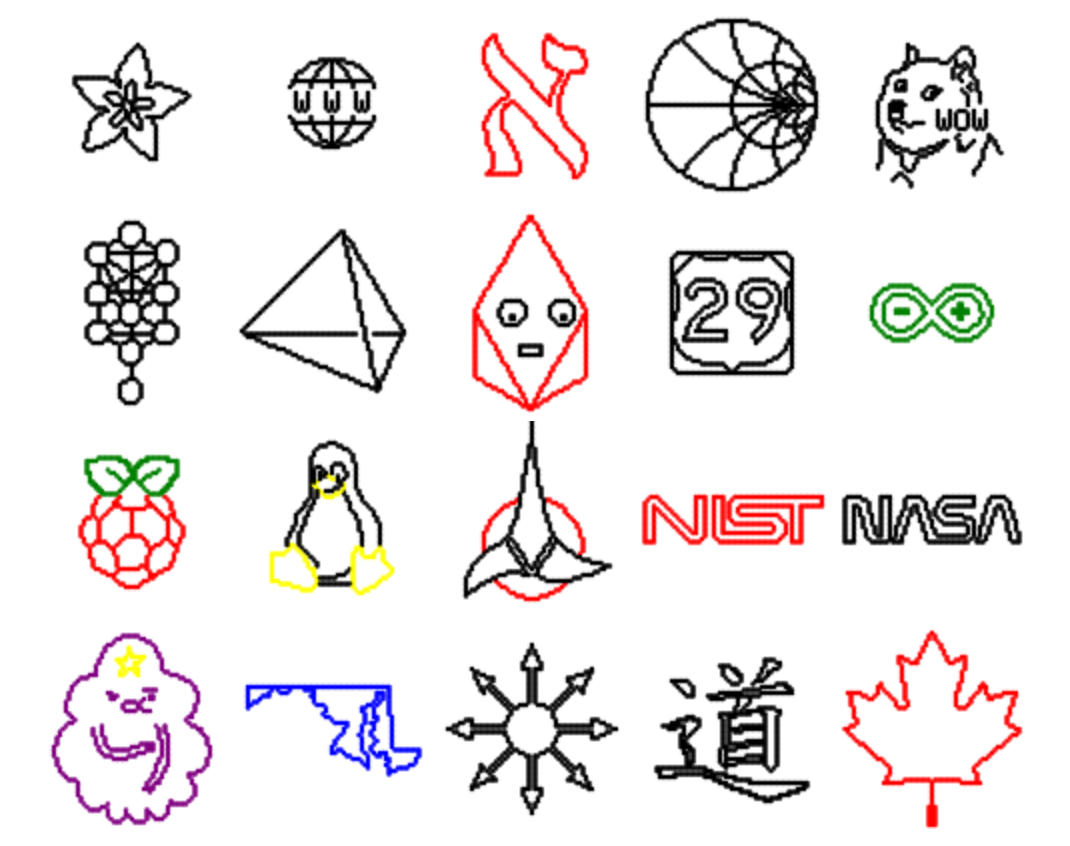
\includegraphics[width=3in]{figures/machines/iconfeed.png}
	\caption[iconfeed]
	{Icon Feed.  Icons are just little bits of text, strings of numbers which are addresses in the Hypercube.  Clicking an icon loads a glyph, which can be copy and pasted. New glyphs can be put in the text area and }
\end{figure}

The Icon Printer framework provides the basis for a very general way to represent any idea with self-replicating physical geometry.  We will discuss in a future chapter how this can be a powerful tool for replication in the most general possible sense.  With the abstraction of the 8 basic pixel movements fixed, this can also be realized in numerous systems besides the ones we have already shown which are included with the Scrolls.  Two such potential versions are to go way up in scale and way down in scale.  At the scale of a whole building, we can use trash-scavenged motors to build a system by which a little cart is pulled side to side along the edge of the roof of the building, which is controlled by one motor controller, and then a rope hoist which controls a winch which pulls a tool up and down along the face of the building.  A can of spray paint is then added to the tool, with a simple mechanism to either engage it or not to draw a paint pixel.  Once the motor controllers are set up to move along the basic 4 directions with or without a pixel, an Icon glyph can be loaded into the controller and an icon can be sprayed on the wall of a building at the scale of meters or 10's of meters.  This might work better on the side of a dumpster or garage door.  Scaling way down can be done either with electron beam lithography or optical lithography using the fine motions on the DVD drive stages.  Lithography is carried out on polished brass, etching away metal everywhere but the pixels using a negative resist.  Some kind of thick material like silicone can then be spun on the brass and then peeled off, making a copy of the icon.  That process can be repeated many times, making in principle an endless feed of copies from the one brass original print.  If this is in a clear material, it can then be put on a surface face down and the patterns will be visible.  This can be used to print text, which can then be read with a scanning optical microscope connected to a cell phone camera, where the mechanical stage for that is also built from trash.  


\begin{figure}
	\centering
	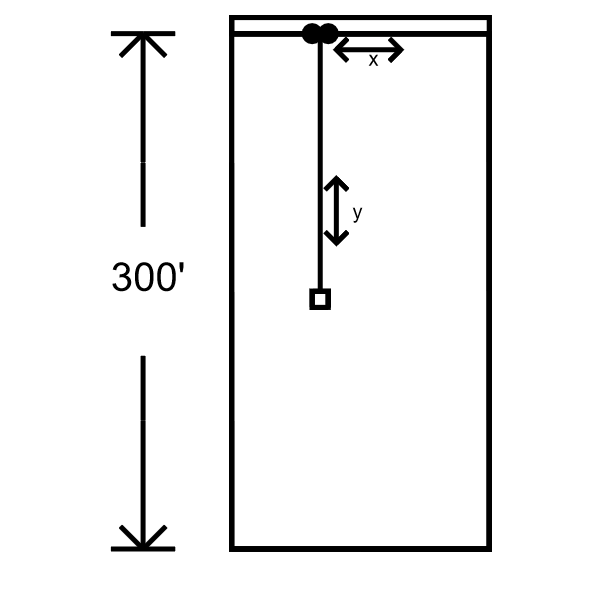
\includegraphics[width=3in]{figures/machines/buildingwallrobot.png}
	\caption[buildingwallrobot]
	{A hoist run along a rail going across the edge of a roof of a building can make a simple robot which can move to anywhere along the wall.}
\end{figure}

\begin{figure}
	\centering
	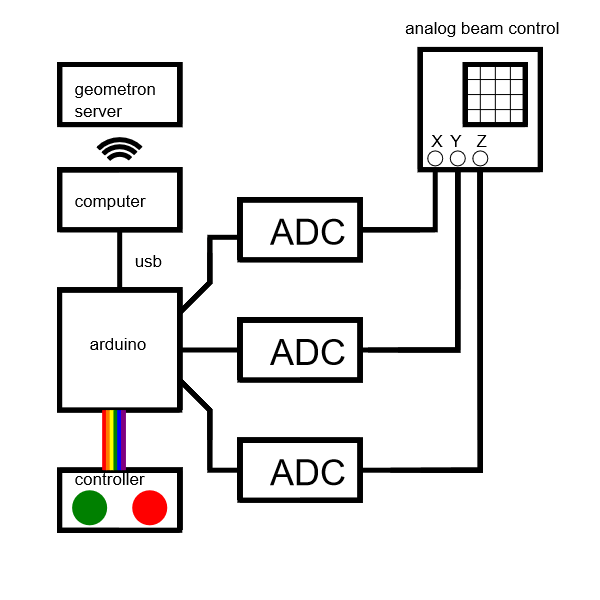
\includegraphics[width=3in]{figures/machines/eblblockdiagram.png}
	\caption[eblblockdiagram]
	{Block diagram of electron beam lithography Geometron robot.  The Arduino here drives three analog to digital converters.  Again the user can design a program for the beam path in a web browser using any computer, which can then also control and power the Arduino and its accessories.  In this case the controller only needs one huge green go button and one huge red stop button.}
\end{figure}


In all cases, we use the Arduino as the basis for the controls.  This versatile free and open platform can be controlled from the Raspberry Pi, meaning that we can have the full automation and printing system along with the server all be self contained without using any private machines.  Thus the printers of self-replicating media can be freely distributed over the Street Network, and anyone can create these and replicate them anywhere, and then share with anyone anywhere else in the world by a simple text message! This is truly a generalized information network.  Any abstract concept can be reduced to a symbol icon glyph.  That glyph can be instantly shared via text message with any of billions of people, and if they have a copy of our self-replicating server with our self-replicating software and our self-replicating robot built from trash, they can make a copy of the icon which is then itself self-replicating physical media.  That can be used by them to communicate any concept in the most abstract possible sense to anyone else.  They can then edit and remix the symbol indefinitely, and share it along with others and so forth.

The prints, stamps, and colorized icons described above are all carried around in black cloth bags.  In addition, the stamps can be used to make pendants with holes at both ends that can be threaded onto Trash Ties from Action Geometry, making another attractive and independent form of personal wearable media which can be integrated into our system.


\begin{figure}
	\centering
	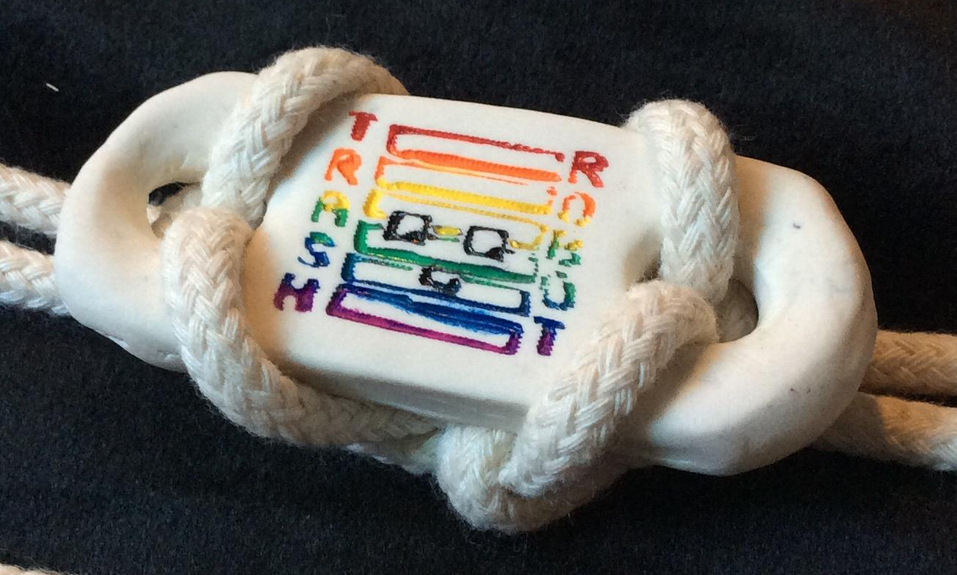
\includegraphics[width=3in]{figures/machines/pendant.png}
	\caption[pendant]
	{Pendant.  One print can make many stamps, one stamp can make many of these.  The back could also be unpainted for easier replication, making the object itself fully self-replicating media.}
\end{figure}
